\chapter{Earth System Models}\label{chapter7}
Earth System Models have evolved from basic atmospheric simulations to complex integrated frameworks that include oceans, land, vegetation, and greenhouse gases. These models are essential for understanding the nonlinear dynamics of climate change and for making reliable projections about future conditions. By incorporating both natural and anthropogenic forcings, ESMs provide a robust tool for addressing pressing questions about climate variability and potential future scenarios.

Until recently, climate studies have predominantly relied on atmospheric models, with only preliminary experiments involving ocean models. However, the significant influence of sea surface temperature (SST) on atmospheric processes required the integration of ocean models with atmospheric models. This coupling led to the emergence of Earth System Models (ESMs), which aim to simulate the dynamic interactions between various components of the Earth system. Early models considered vegetation and certain atmospheric gases as external forcings. However, as climate science advanced, external forcings were redefined to include anthropogenic influences such as greenhouse gas concentrations, while other previously external factors, such as ocean dynamics, became integral components of the coupled model.
For example, $CO_2$ is well-mixed in the atmosphere, meaning its concentration is nearly uniform globally. $CO_2$ is a major contributor to radiative forcing, with approximately 58\% of the radiative effect attributed to it.
Quantifying the increase in $CO_2$ requires models capable of simulating its interactions with the ocean, land, and atmosphere. In this model SST should not be considered as external forcing, that now becomes the $CO_2$.

\begin{figure}[htpb]
    \centering
    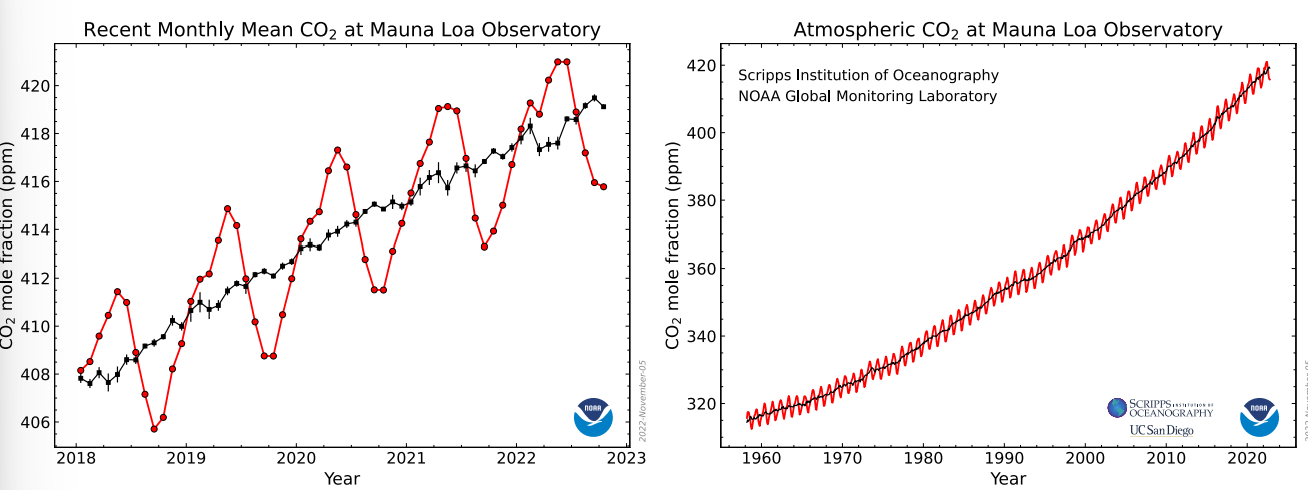
\includegraphics[width=0.5\linewidth]{uploads/co2image.png}
    \caption{Monthly mean $CO_2$ at Mauna Loa}
 
\end{figure}
Methane ($CH_4$) emissions are increasing and measured in parts per billion. Unlike CO$_2$, which is mainly emitted from combustion processes, CH$_4$ emissions arise from livestock (for example, cattle farming), agricultural practices (for example, rice paddies), and industrial activities, including leaks in extraction industries.
\begin{figure}[htpb]
    \centering
    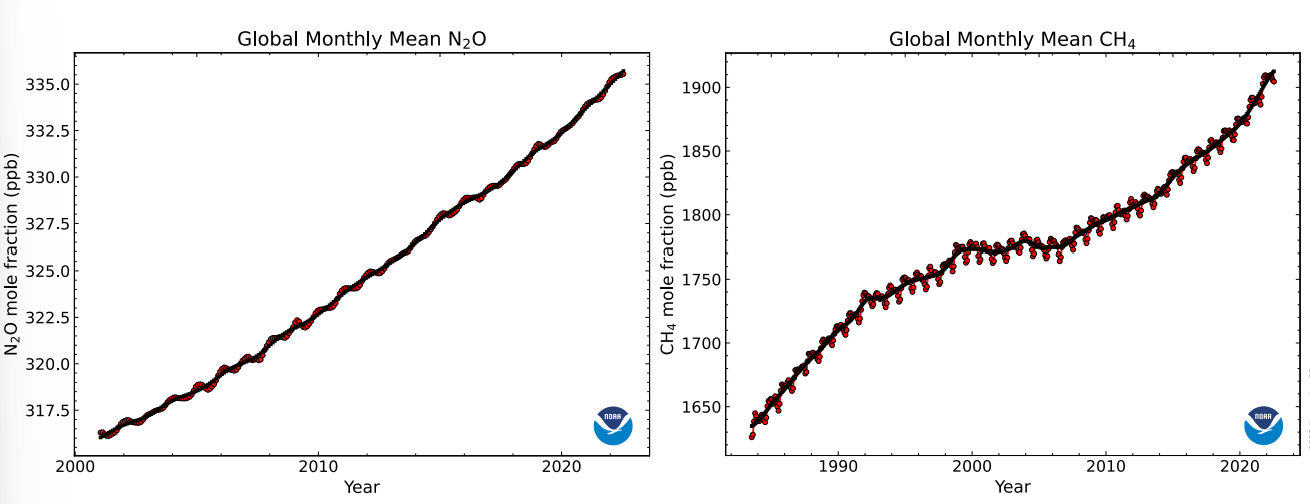
\includegraphics[width=0.5\linewidth]{uploads/ch4.png}
    \caption{Emissions of $CH_4$ in part per billion.}
   
\end{figure}
Ice cores provide critical data on past climate oscillations, revealing historical CO$_2$ and CH$_4$ concentrations. These records show the natural variability of greenhouse gases over millennia, serving as a baseline for assessing the impacts of recent anthropogenic emissions.\\




To project future climate conditions, models incorporate assumptions about socioeconomic scenarios that dictate greenhouse gas emissions. Stone and Weaver\cite{Stone2000} work highlighted that climate change would not merely shift temperature distributions but would fundamentally alter their characteristics, leading to nonlinear alterations, underscoring the need for comprehensive modeling frameworks.

\begin{figure}[htpb]
    \centering
    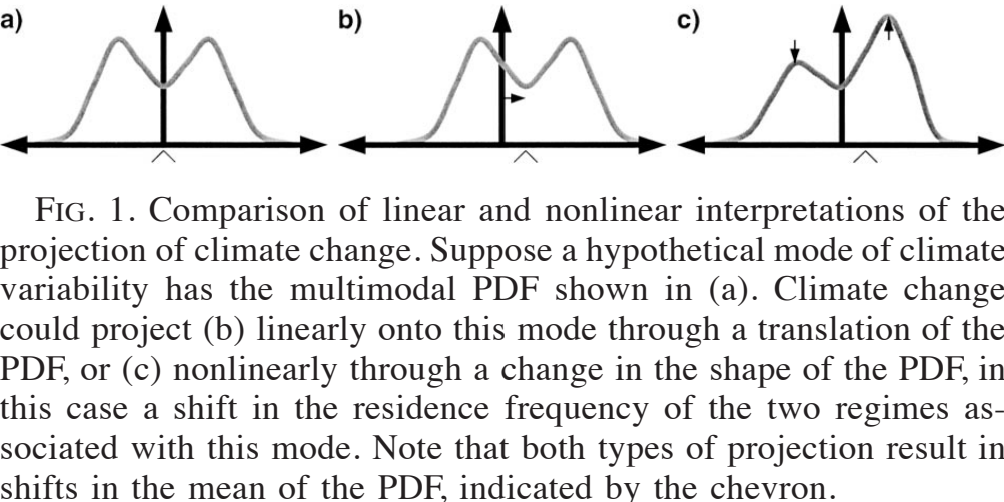
\includegraphics[width=0.5\linewidth]{uploads/nonlinclimatechange.png}
    \caption{Comparison on linear and nonlinear interpretations of the projection of climate change.}
    \label{fig:clim model}
\end{figure}
In the fig\ref{fig:clim model} a) represents a situation where warm and cold temperatures are equiprobables, b) redefines what is cold or warm, c) climate change will displace much more warmer than colder over the year.

\section{Expectations with increasing greenhouse gases}
Climate projections often begin with control runs: 
\begin{enumerate}
    \item initialization: start with current atmospheric $CO_2$ levels. This is also referred to as \textit{control run} (reference experiment). A baseline simulation under current climate conditions, ensuring initial energy balance in the system.
    \item Incremental forcing: increase $CO_2$ concentration by 1\% annually until it doubles or quadruples relative to the baseline (2xCO$_2$, 4xCO$_4$). This is referred to as a \textit{perturbation experiment}, introducint changes and allowing the system to evolve until the new equilibrium is reached, tracking the stabilization process, ensuring that energy balances across the system.
    \item Equilibrium simulation: run the model until a stable equilibrium is reached, ensuring the ocean and atmosphere are in balance: the system must stabilize energetically. This avoids "drift," where the model might otherwise converge toward unrealistic or biased states. The atmosphere typically stabilizes more quickly, while ocean circulation requires longer timescales, often 4 years to stabilize circulation. 
\end{enumerate}
Predictive models requires accurate initial conditions obtained
from observations via constrained estimation methods “data
assimilation”. Climate models requires equilibrated atmosphere and ocean, therefore a spin-up period is usually used. Spin-up is the time taken for an ocean/atmosphere model to reach a state of statistical equilibrium under the applied forcing.\\


Increasing greenhouse gas concentrations enhance atmospheric opacity, trapping more longwave radiation. This effect leads to a rise in surface temperatures, what about the other variables?

Changes beyond surface warming will change the character of climatic fluctuations, not just the mean temperature (panel c) of \ref{fig:clim model}. This includes shifts in the distribution and variability of other variables, such as precipitation and atmospheric circulation.



Analyzing changes in variability is crucial. For example, EOF analysis is used to identify dominant modes of variability within the control integration. This helps differentiate natural variability from anthropogenic impacts.
\paragraph{Characteristics of warming}
Warming is more pronounced in polar regions due to feedback mechanisms like ice-albedo interactions and changes in heat transport. Land areas warm faster than oceans due to lower heat capacity and less mixing compared to water bodies. Oceans act as heat sinks, absorbing significant portions of excess energy. However, this occurs over longer timescales, delaying the full extent of warming. Surface warming occurs rapidly on land and polar regions, while oceanic warming unfolds over decades or longer.

\begin{figure}[htpb]
    \centering
    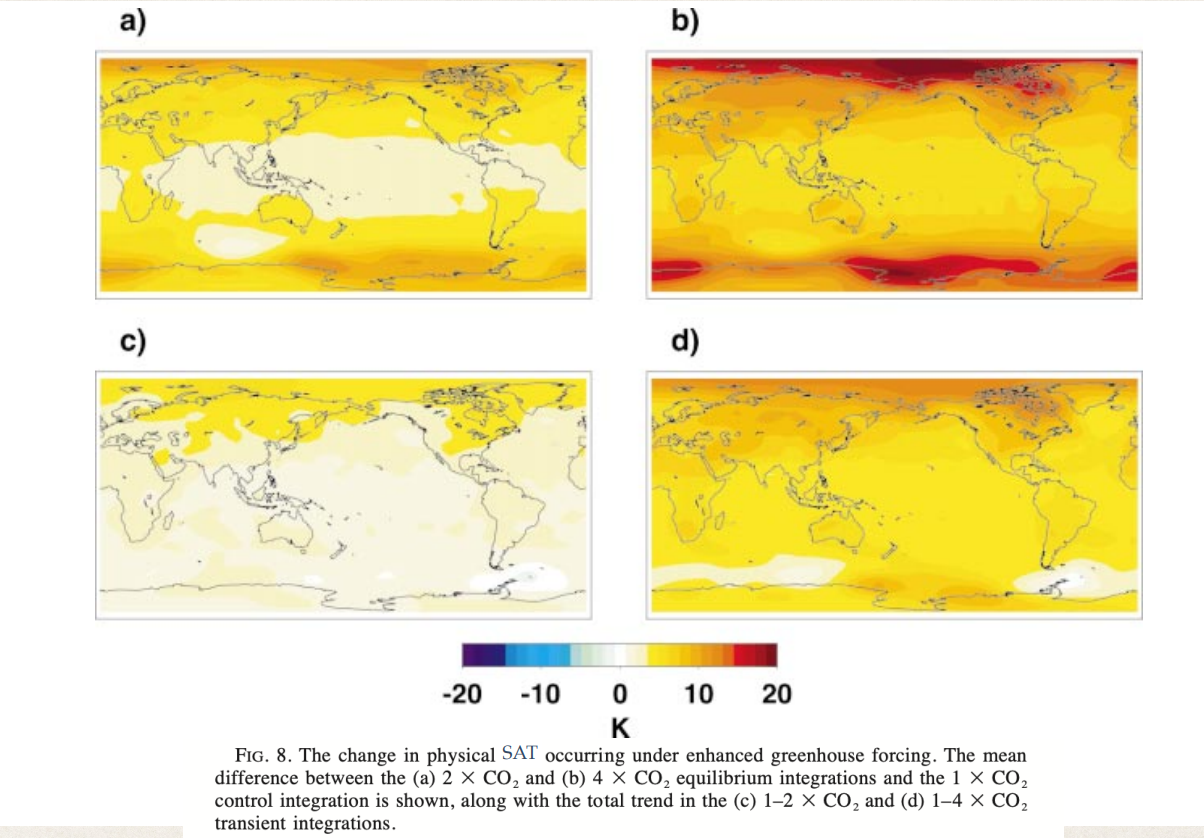
\includegraphics[width=0.5\linewidth]{uploads/imagewarming.png}
    \caption{One of the first evidence to the distribution of warming.}
    \label{fig:warming}
\end{figure}

Model outputs often present: 
\begin{itemize}
    \item Control run variability: baseline distributions of temperature, precipitation and other variables to compare against perturbed states. 
    \item Amplification and shifts: evidence of stronger warming trends over polar regions and continents 
    \item Ocean response: visual representations of delayed oceanic warming compared to surface or land responses.
\end{itemize}
\section{Expanding the complexity of climate modeling}
\paragraph{Pioneering exercises in Earth System Modeling} If climate characteristics are changing, it means that the characteristics of vegetation will change. For example, 15 vegetation classifications emerge based on temperature and precipitation. As climate changes, vegetation responses must be integrated into the model. \\

Particles, such as aerosols, also influence temperature and climate. Their effects depend on particle size, with smaller aerosols increasing albedo. Modeling aerosol effects requires intricate calculations and includes microphysics, where microscopic processes play a significant role.

Coupling components at higher frequencies—shifting from daily to hourly exchanges between Earth-atmosphere and ocean-atmosphere—became necessary for accurate simulations. 

\paragraph{Equilibrium climate sensitivity} Equilibrium Climate Sensitivity (ECS) is historically estimated at 2.2-2.5°C, ECS measures the temperature response to CO$_2$ doubling. ECS may evolve with baseline temperatures, complicating future predictions (if climate sensitivity depends on basic temperature, increasing it doesn't mean that climate sensibility will stay the same). However, as baseline temperatures rise, ECS may also evolve, making linear assumptions inadequate. Modern climate projections, driven by socioeconomic scenarios, aim to quantify these nonlinear changes, such as shifts in precipitation patterns (15–20\% increase) and polar amplification of warming.
\begin{figure}[htpb]
    \centering
    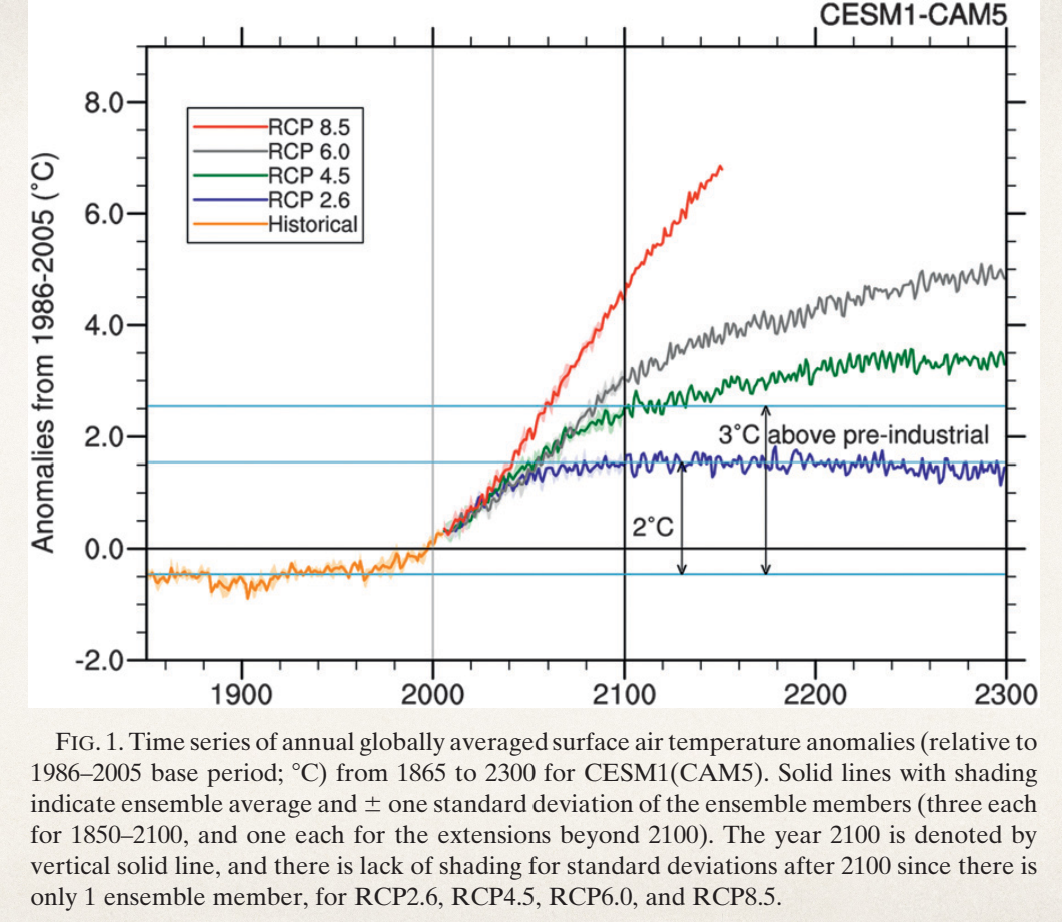
\includegraphics[width=0.5\linewidth]{uploads/climatescenarios.png}
    \caption{Climate scenarios including social economics assumptions}
    \label{fig:clim scenarios}
\end{figure}
\begin{figure}[htpb]
    \centering
    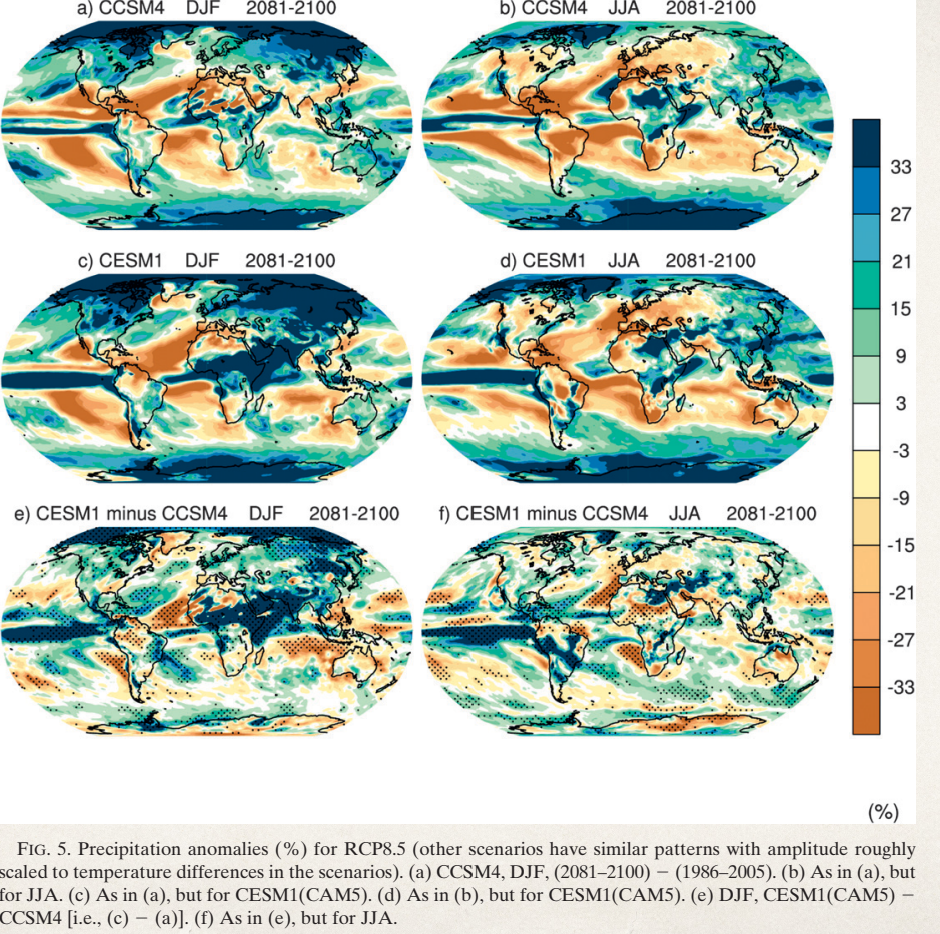
\includegraphics[width=0.35\linewidth]{uploads/precipitations.png}\quad 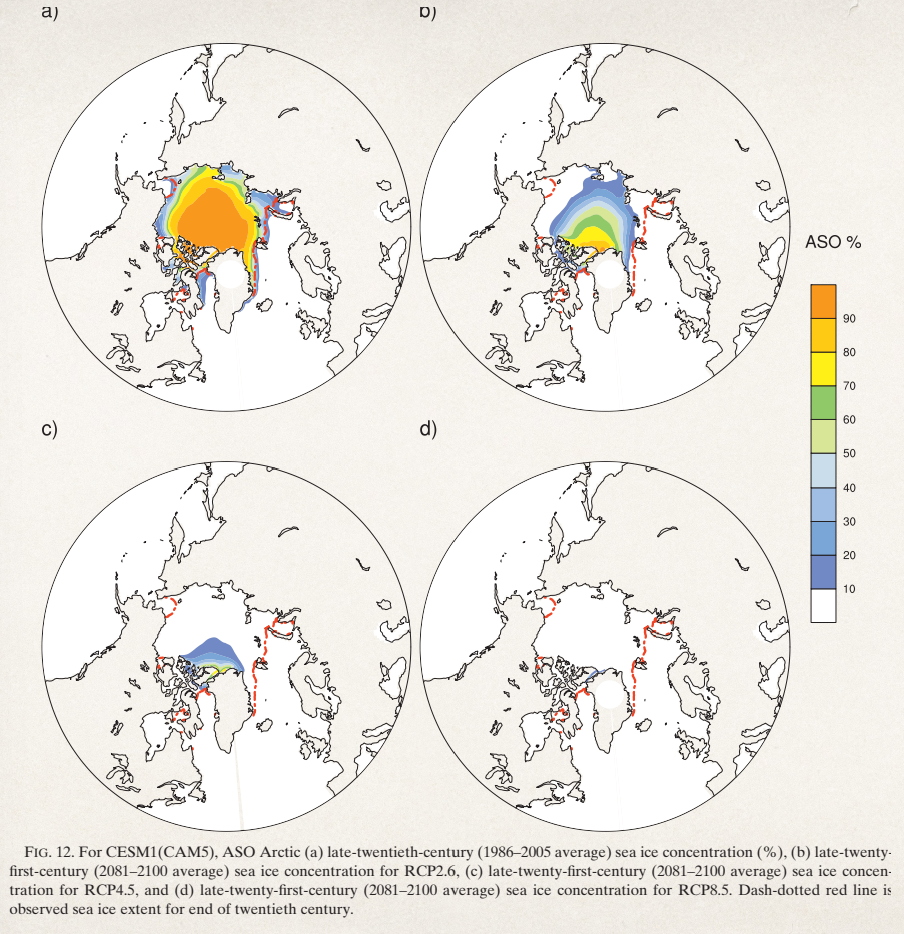
\includegraphics[width=0.35\linewidth]{uploads/sea ice.png}
    \caption{Precipitation anomalies (\%) and sea ice concentrations (\%)}

\end{figure}

\section{Carbon and Biogeochemical cycles} 
Some definitions: 
\begin{itemize}
    \item \textit{Geochemistry:} studies the chemical composition of the Earth and the cycling of its chemical elements and major compounds that circulate between the natural reservoirs of the outer envelope lithosphere, atmosphere, hydrosphere and biosphere.  
    \item \textit{Biogeochemistry: } studies the effects of living organisms on chemical composition and cycling. 
    \item \textit{Biogeochemical cycles:} studies the transport and cyclic transformation of chemical elements (or compounds) inuenced by the activity of living organisms. 
\end{itemize}
\paragraph{Chemical composition of the ocean} The chemical composition of the ocean is driven by air-sea exchange: dissolution in air or in surface waters (where solubility is given by the products of partial pressure and the solubility coefficient, which is different for each gas and de-(in-)creases with in-(de-)creasing water temperature); by atmospheric deposition; by accumulation of terrestrial inputs and by removal through marine sediments. 

\subsection{The Carbon cycle}
Carbon is the defining element of organic matter: virtually all organisms are based predominantly on carbon compounds, it is present in all reservoirs: biosphere, hydrosphere, atmosphere and lithosphere. Atmospheric components CO$_2$ and methane (CH$_4$) are greenhouse-gases, the latter being less abundant (\~100x), but more effective (20x), but also unstable (turnover time \~10y). 
\begin{figure}[htpb]
    \centering
    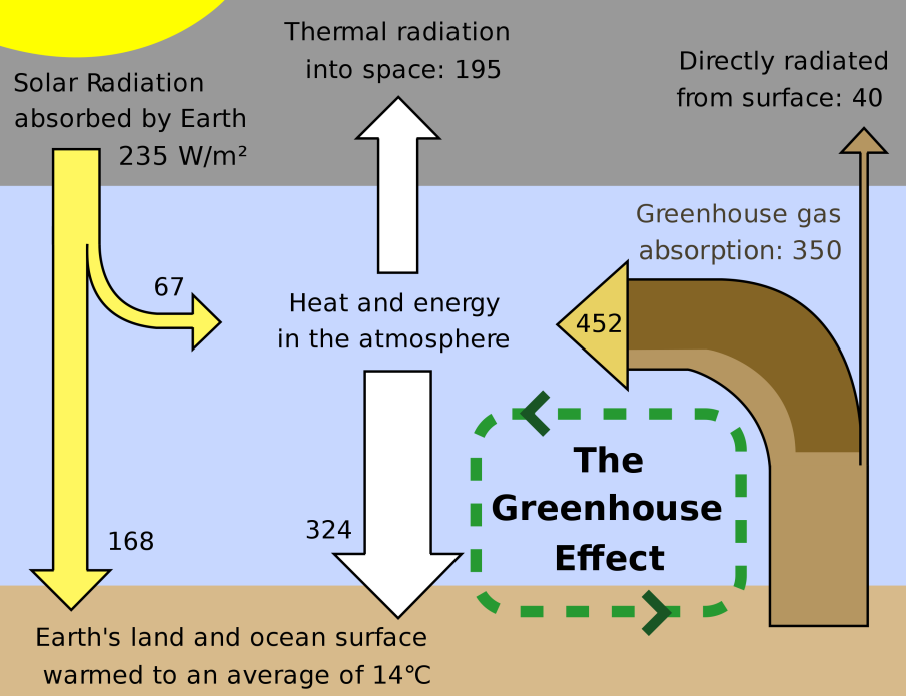
\includegraphics[width=0.4\linewidth]{uploads/greenhouse situa.png}
    \caption{Greenhouse effect affects radiative balance. Greenhouse gases act as external forcing but what we are really interested in are emissions: what percentage of CO$_2$ stays as concentration and doesn't go away in the biological system? What part of these will be absopted, which goes in the biochemical system and so on. 
A certain portion of the emission will be digested by the system, the extra will go into the atmospheric concentration, the net result is to have a model much more difficult to understand and model.}
    
\end{figure}
Carbon is also found in transformed sedimentary rocks from marine sediments. Inorganic forms in the ocean are separated into dissolved (DIC) and particulate (PIC), including calcareous structural material originating from plankton, corals and shells. 

The carbon cycle, an integral part of Earth System Models (ESMs), includes fluxes among the atmosphere, ocean, and land. Carbon dioxide absorption occurs until equilibrium between the atmosphere and ocean is reached. Processes like sediment removal also play roles in long-term carbon storage. Vegetation acts as both a source and a sink for CO$_2$, dynamically interacting with atmospheric concentrations.\\



The interplay of carbon with other cycles (e.g., nitrogen and phosphorus) further complicates these models. The equations governing these systems combine advection, diffusion, and biogeochemical reactions, often expressed as:
$$\frac{\partial C}{\partial t}=\vec{v}\cdot \nabla C=Sources-Sinks$$

\paragraph{Oxygen cycle}
Oxygen is the most abundant
element in the Earth’s crust and
second most abundant in the
ocean. Its presence is due to imbalance of
photosynthesis and respiration,
guaranteed by the deposition of
organic compounds in sediments,
where they can not be oxidised. Oxygen is toxic to anaerobic
organisms and at high concentrations even to aerobic ones. Cyanobacteria were the first organism to perform photosynthesis, in the "Great Oxygenation Event". Oxygen is produced by the splitting of the water molecules in photosynthesis, approximately half of this production occurs in the ocean. Dissolved oxygen supply is high
in the surface ocean due to air-sea exchange and
photosynthesis. It is reduced in the intermediate layer due to consumption, particularly at low to mid latitudes. It generally increases again in the deep ocean where it is supplied by deep water
formation and barely consumed.\\
[0.2cm]


Subtropical gyres, vast regions of rotating ocean currents, are often described as the deserts of the ocean due to their low biological productivity. These gyres are characterized by warm, nutrient-poor waters that limit phytoplankton growth and, in turn, reduce the primary production essential for sustaining marine food webs. Despite their low productivity, these regions play a significant role in global biogeochemical cycles by acting as carbon sinks, absorbing atmospheric CO$_2$ and sequestering it in the ocean interior over long timescales.\\

Ocean acidification, a direct consequence of increasing CO$_2$ concentrations, poses a profound threat to marine ecosystems, including those in subtropical gyres. As the ocean absorbs more CO$_2$, it forms carbonic acid, lowering the pH of seawater and increasing its acidity. This shift affects the carbonate chemistry of the ocean, impairing the ability of calcifying organisms, such as corals and certain plankton species, to build and maintain their calcium carbonate structures. Warm-water corals, for instance, are particularly vulnerable; when combined with rising temperatures, acidification leads to widespread coral bleaching and mortality.




These changes are not uniform and depend on regional factors, but the overall trend toward more acidic and nutrient-depleted subtropical gyres highlights the intertwined impacts of climate change on ocean dynamics and marine life. Understanding these processes is essential for predicting the future health of ocean ecosystems and their role in regulating Earth’s climate.\\
[0.2cm]

There's a wide range of approaches to the marine ecosystem models, such as eulerian/lagrangian modelling, individual based models, food-web models, dynamic size spectrum models and so on. \\

We can write a more detailed dynamic equation for biogeochemical tracers, as the change of biogeochemical concentrations in the ocean interior is given by: advection, diffusion (turbulent and molecular, the latter is usually neglectible), biogeochemical sources and sinks (production, losses, vertical movements: 
\begin{equation}
    \frac{\partial C}{\partial t}=-\vec{v}\cdot\nabla C+K\nabla^2 C+\frac{\partial C}{\partial t}\big|_{bgc} 
\end{equation}
in its simplest form, biogeochemical changes are assumed proportional to the tracer concentration, where $r$ may be a function of other state variables:
$$\frac{\partial C}{\partial t}\big|_{bgc} =rC$$


An \textbf{Earth System Model (ESM)} needs to take into account atmospheric dynamics, ocean dynamics, cryosphere, hydrography, atmospheric chemistry, terrestrial ecosystem, marine ecosystem. 
\begin{figure}[htpb]
    \centering
    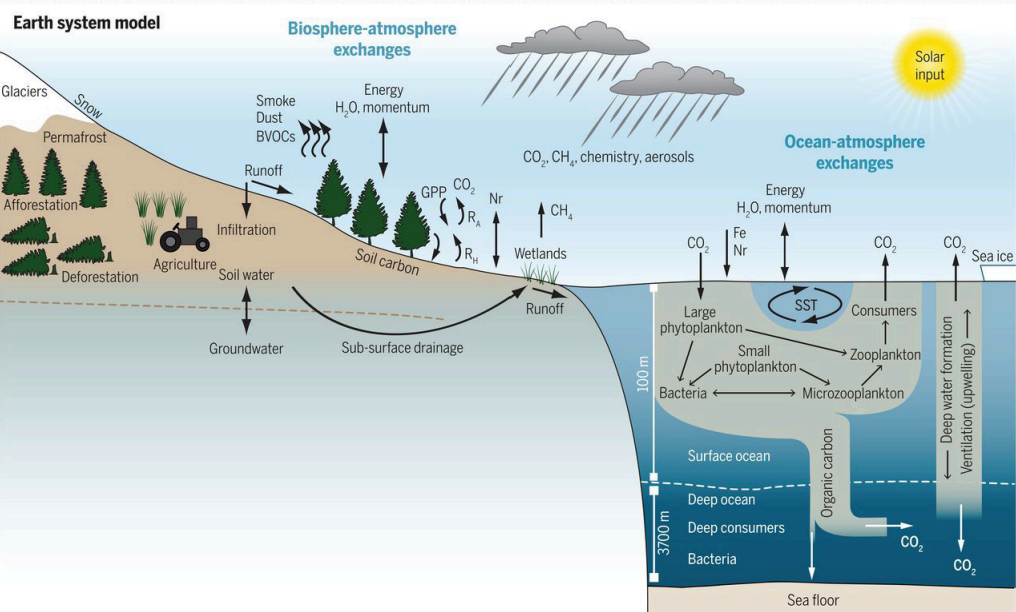
\includegraphics[width=0.5\linewidth]{uploads/Earth system model.png}
    \caption{Earth system model}
   
\end{figure}

\subsection{Complexity and model evaluation}
Advancements in ESMs have dramatically increased complexity due to:
\begin{enumerate}
    \item Higher resolution (spatial and temporal, horizontally and vertically), enhancing model accuracy but demanding greater computational resources: more variables to compute, but increasing resolutions means more degree of freedom. 
    \item Inclusion of biogeochemical tracers for carbon, nitrogen, and phosphorus cycles.
    \item Expanding interactions among components like sea ice, topography, and biological systems.
\end{enumerate}
Model performance is evaluated against satellite observations, revealing improved simulation fidelity over time, especially in capturing chlorophyll distributions and carbon fluxes.
\begin{figure}[htpb]
    \centering
    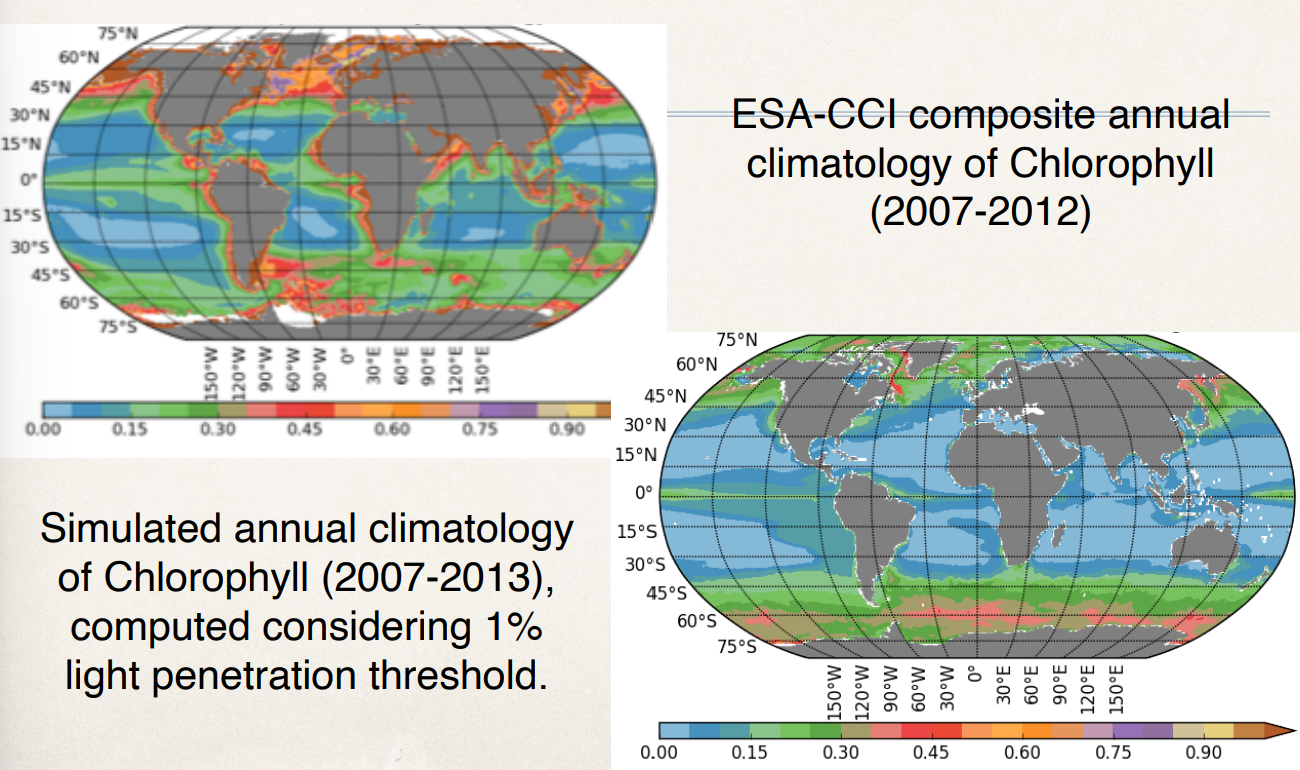
\includegraphics[width=0.4\linewidth]{uploads/goodmodels.png}
    \caption{How good are these models, from satellites (left) and model (right).}
 
\end{figure}


Efforts like the CMIP6 project coordinate global climate scenarios, extending from pre-industrial times (850 CE) to future projections (2100 CE). These simulations consider volcanic eruptions, orbital variations, historical land-use changes.
Models predict that both land and ocean systems, traditionally acting as carbon sinks, may transition into sources as emissions continue. These insights highlight the necessity of understanding and mitigating anthropogenic impacts on Earth's climate systems.
\begin{figure}[htpb]
    \centering
    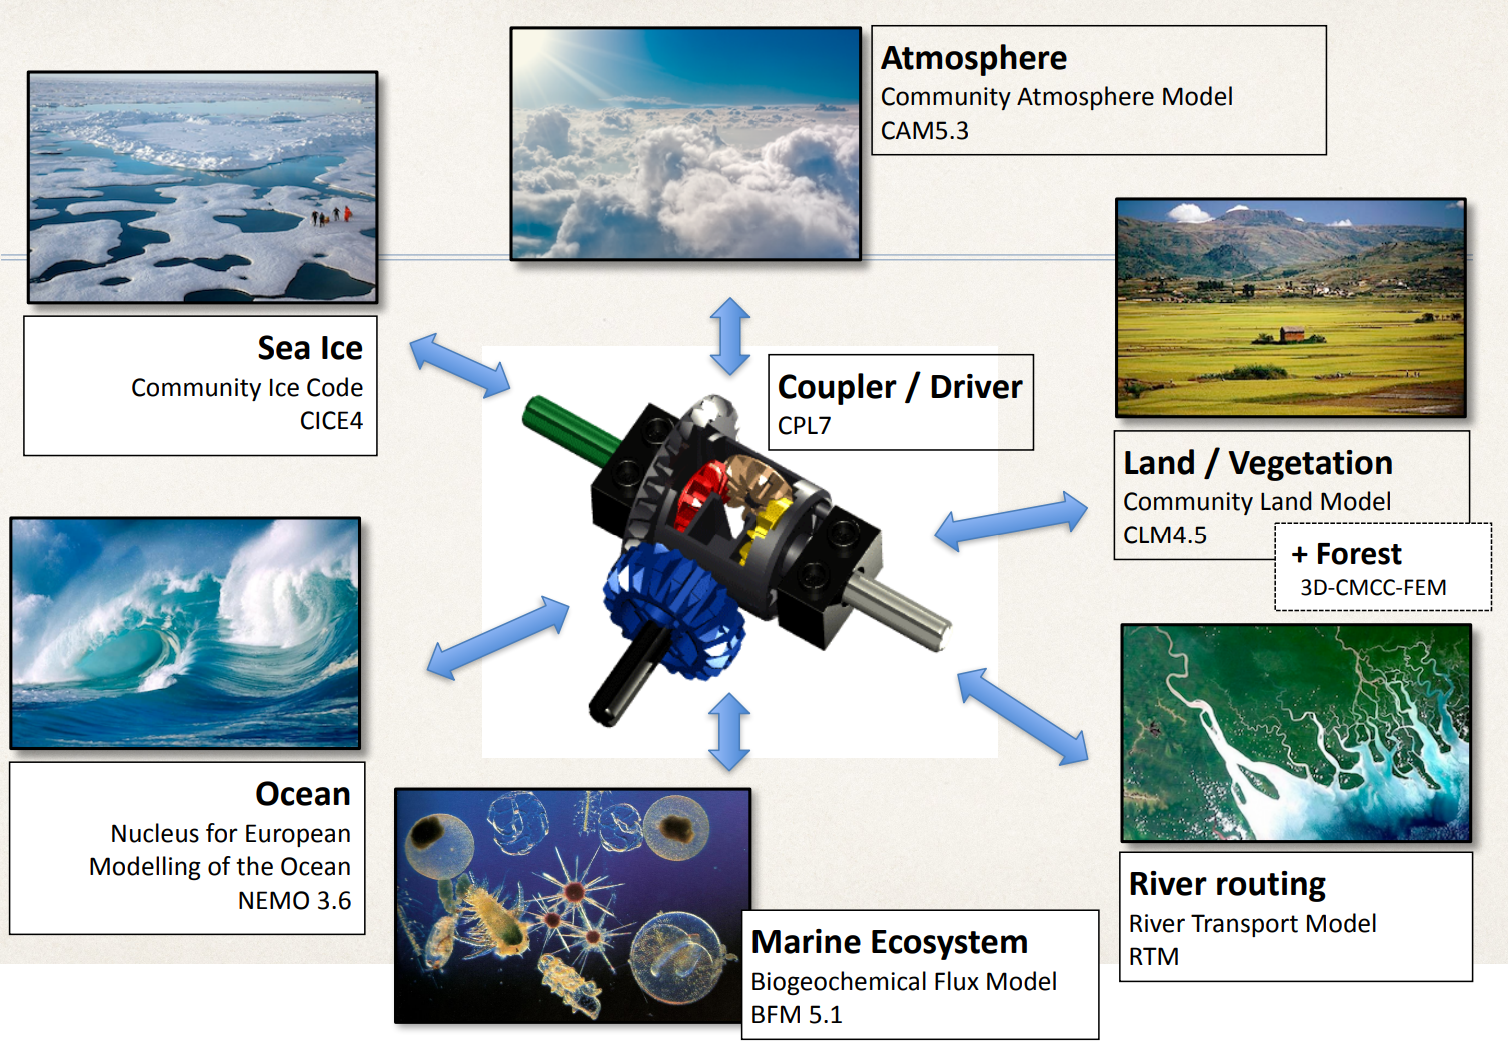
\includegraphics[width=0.4\linewidth]{uploads/CMCC model.png}
    \caption{CMCC Earth System model for CMIP6}

\end{figure}

\begin{figure}[htpb]
    \centering
    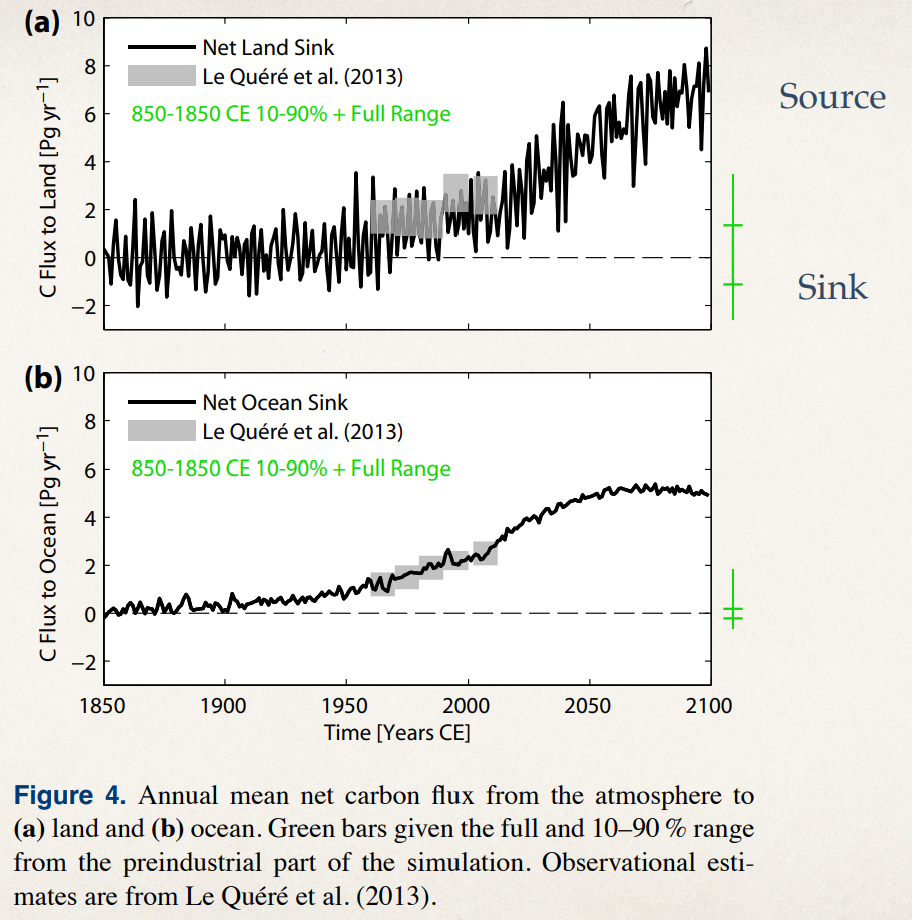
\includegraphics[width=0.5\linewidth]{uploads/sources.png}
    \caption{Fluxes of carbon between ocean and land, if above $0\rightarrow$ source. In this model both land and ocean become sources of carbon fluxes}

\end{figure}
In climate system modeling, one of the primary tools is the 3D model that provides a comprehensive representation of various environmental systems. This model allows us to observe what happens in different regions of the Earth, including complex areas like the deep ocean. A challenge in working with these models is identifying patterns, as each component—whether species, ecosystems, or regions—follows unique behavior or patterns. These patterns can vary significantly, making it difficult to predict or generalize. However, once these patterns are understood, we can better strategize interventions or "fixes" to mitigate negative effects.

Since climate models often involve simulating multiple scenarios based on different assumptions and variables, it's essential to consider a variety of possible outcomes. One key measure in these simulations is radiative forcing, a value that quantifies the energy imbalance in the climate system caused by factors like greenhouse gas emissions. The radiative forcing value for each scenario is represented by the last two digits (e.g., \textbf{0.36}, \textbf{0.41}, etc.), which correspond to specific scenarios or pathways of emissions. Even though many combinations of factors may lead to the same radiative forcing value, understanding how these different scenarios play out is crucial in assessing their impacts.

A significant factor in determining the outcomes of climate models is the amount of \textbf{greenhouse gases (GHGs)} in the atmosphere. The more GHGs present, the stronger the overall climate response. For example, the \textbf{RCP 2.6} scenario, which involves significant emission reductions, requires \textbf{negative emissions} (i.e., removing carbon from the atmosphere) after 2050–2060 in order to limit global temperature increases to \textbf{2°C}.
\begin{figure}[htpb]
    \centering
    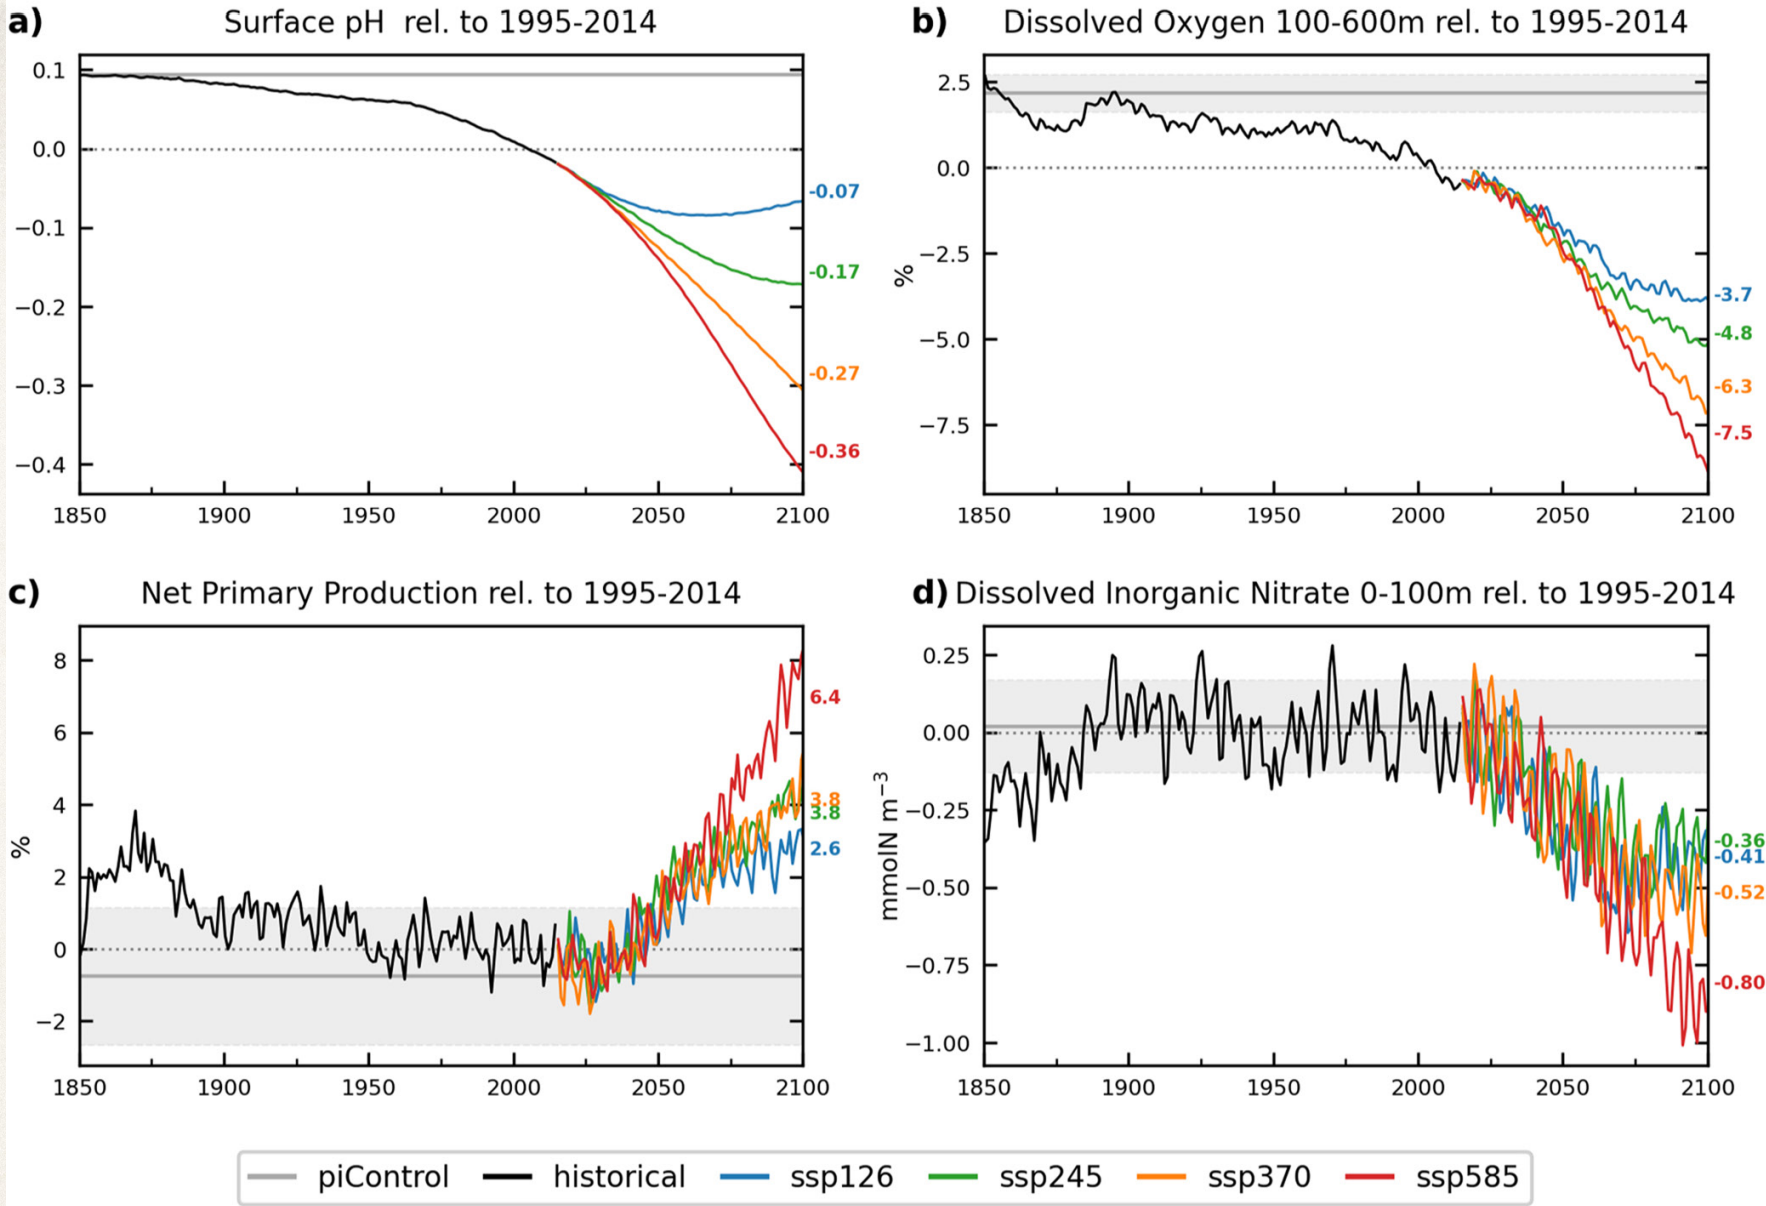
\includegraphics[width=0.5\linewidth]{uploads/predictions.png}
    \caption{Models and predictions}
    
\end{figure}

One of the direct consequences of global warming is the increase in temperature, which affects various oceanic processes. For example, an increase in temperature can lead to a decrease in dissolved oxygen levels in the ocean. Warmer waters can hold less oxygen, which has serious implications for marine life. Additionally, nitrate levels are expected to decline due to changes in the ocean's biological production. The reduction in nutrient availability results in lower oxygen production, further exacerbating the oxygen depletion in marine ecosystems.

\paragraph{Equilibration and Feedbacks}

In equilibration experiments, we simulate the effects of stopping emissions and assess how the system reacts. For instance, if emissions were to stop, the concentration of greenhouse gases in the atmosphere would stabilize, and the system would eventually reach a new equilibrium. However, it takes time for the temperature to stabilize, and there is typically a time lag of 10–15 years before equilibrium is reached. The full impact of warming may take 15–20 years to manifest, reflecting the cumulative effect of past emissions. This delay is akin to a Green's function, where the system's response to a perturbation is integrated over time.

This phenomenon of committed warming means that even if emissions were reduced immediately, the Earth would continue to warm for some time due to the inertia in the climate system. Ensemble runs are often used in these experiments to explore a range of possible outcomes, with each run representing a different set of initial conditions or assumptions.

\begin{figure}[htpb]
    \centering
    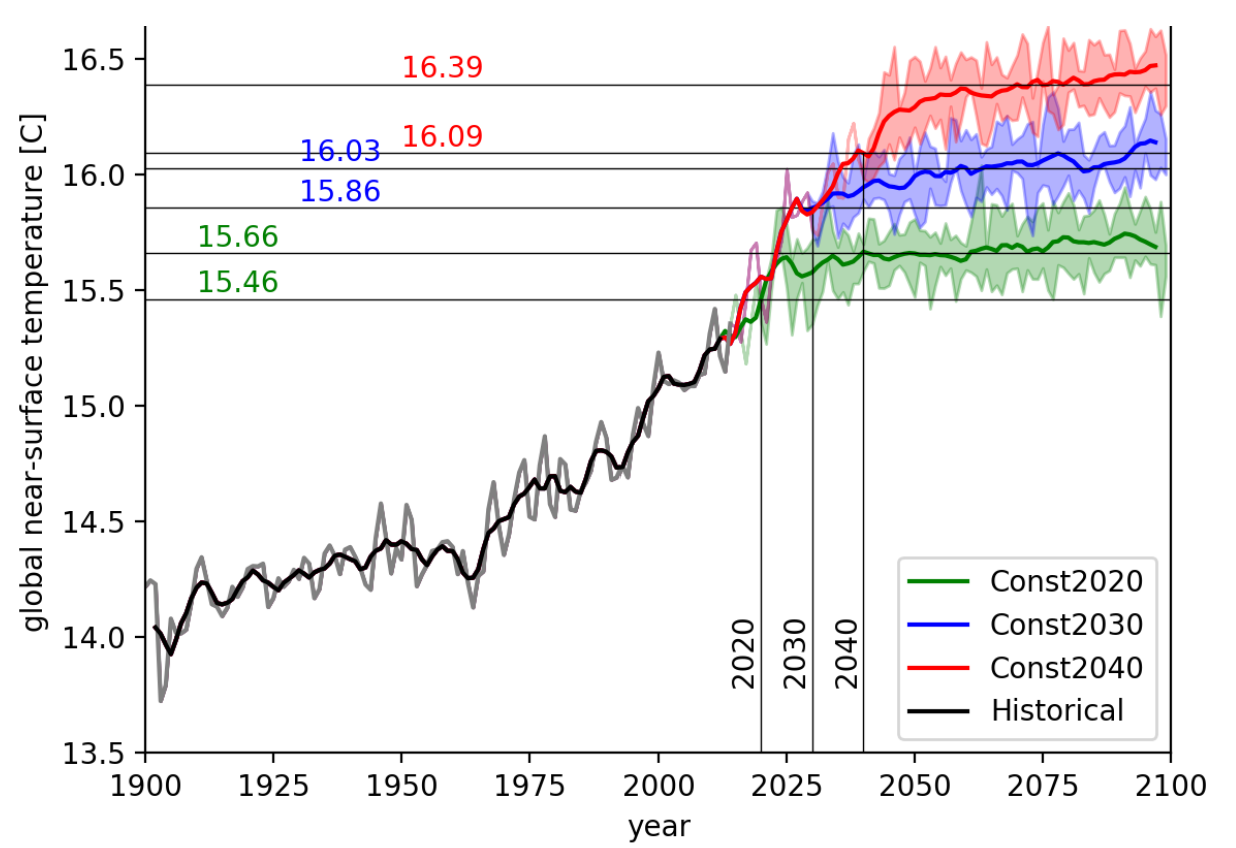
\includegraphics[width=0.5\linewidth]{uploads/eqexperiments.png}
    \caption{Equilibration experiments}
    
\end{figure}


\section{Digital Twins}
The concept of Digital Twins has gained significant popularity in recent years. A digital twin is a virtual model of a physical system, designed to simulate and predict the behavior of that system. This approach is increasingly used in fields like climate modeling to understand complex processes without needing direct physical experimentation. The idea is to create an interconnected feedback loop where the digital model receives real-time information from the physical system, allowing for better prediction and control.


A \textit{digital model} serves as a mathematical representation of a physical system informed by real-world data and experiments. These models aim to produce predictions that closely align with actual observations, improving forecasting capabilities and providing a more accurate representation of the Earth’s systems. A \textit{digital shadow} represents the continuous real-time data flow that informs and updates the model.

In contrast, a digital twin is a completely integrated system, it goes beyond just simulating behavior; it integrates real-time feedback and allows for some level of control over the physical system. However, when it comes to the Earth system, we are still far from achieving a fully integrated digital twin due to the sheer complexity and scale of the planet’s processes.

\begin{figure}[htpb]
    \centering
    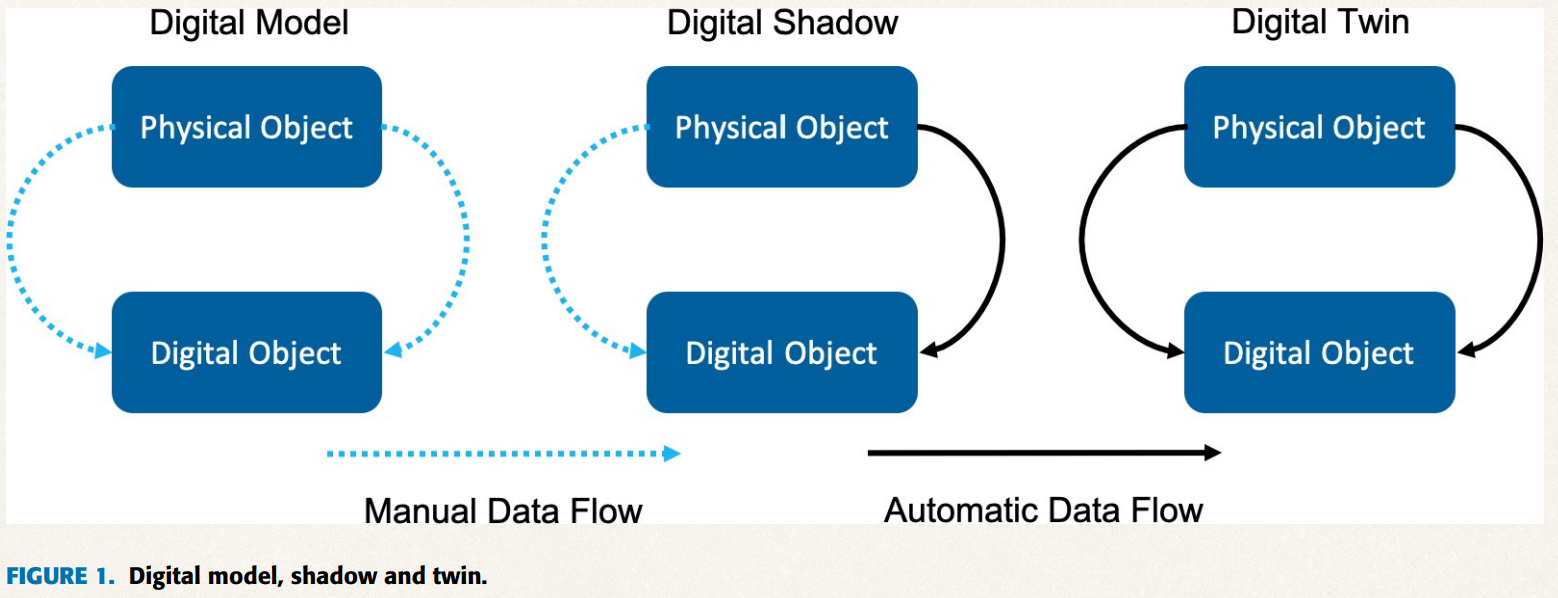
\includegraphics[width=0.5\linewidth]{uploads/digital twins.png}
    \caption{Digital world}
    
\end{figure}

\subsection{Enabling Technologies}
Climate modeling increasingly relies on enabling technologies—tools and innovations that enhance the ability to model complex systems. These technologies might include new ways of gathering observational data, improving the accuracy and resolution of models, or developing better computational methods for simulating climate processes. Unlike basic knowledge, enabling technologies facilitate progress by providing the infrastructure and tools needed to make climate predictions more accurate and actionable.

One focus is the use of non-conventional sources of observation. Traditional data sources like ground-based measurements or satellite observations are valuable but may have limitations. By exploring new types of observations, such as those from new sensors or alternative platforms, we can improve the quality of the models and increase their robustness.

\section{Climate Ensembles}
In climate modeling, we work with ensemble models, which involve running simulations under different initial conditions and assumptions. Given that there is inherent uncertainty in predicting the exact future state of the climate, these ensembles help capture the range of possible outcomes.

One of the key challenges is understanding and managing the uncertainty that comes with internal climate variability. While external factors like greenhouse gas emissions are relatively predictable, internal variability (e.g., ocean currents, volcanic activity) is much harder to forecast accurately. This uncertainty affects the predictions, and we typically express it in terms of standard deviation within the ensemble. The spread in the model outputs reflects the uncertainty in predicting specific outcomes, such as temperature rise or the rate of ice sheet melting.



The uncertainty surrounding climate sensitivity—the Earth's response to changes in greenhouse gas concentrations—is a significant factor in climate projections. Even though we have a general idea of the climate's response, there are still unknowns, particularly when it comes to regional effects or extreme events. This uncertainty is not just physical, but also depends on the emission scenario chosen. Different emission pathways lead to different climate futures, making the exact trajectory difficult to pin down. Some models predict rapid warming, while others may show slower changes, reflecting this uncertainty.



Ultimately, the challenge of climate modeling goes beyond just predicting specific scenarios. It's more about understanding \textbf{climate risks}—the potential for large-scale, unpredictable changes that could result from different emission scenarios. While we can predict trends like ice sheet melting or temperature increases, the exact timing and scale are much more difficult to determine. The unpredictability of these changes makes climate risk a significant concern, and it highlights the importance of uncertainty management in climate modeling.


 
